

As has already been pointed out,
both the computation of moments and probabilities reduces to numerical
integration, and a dominant technique for doing this is Monte Carlo simulation.
The approximate computation of expectation
$E[\chi_\phi \cdot (h \circ t)]$,
\begin{equation}
\frac{1}{n} \cdot \sum_{i=1}^n p(\vec{x}_i) \cdot \chi_\phi(\vec{x}_i) \cdot
h(t(\vec{x}_i)),
\end{equation}
faces a number of difficulties.
This section describes how these are addressed in PIP.

{\bf Basic sampling from $p$}.
It may be hard to sample from $p$.
Pip implements MCMC (in the form of the Metropolis algorithm),
a very powerful and general technique for computing samples, essentially based
on random walks in a Markov Chain biased by $p$. Of course, this technique
has a considerable overhead and is avoided where possible.

{\bf Independent random variables}.
In many special cases, there are better techniques, such as
when the random variables are mutually independent (i.e.,
$p_{X_1 \dots X_k}(x_1, \dots, x_k) = \prod_{i=1}^k p_{x_i}(x_i)$).
In that case, we sample independently from the various constituent
distributions $p_{X_i}$.  It should also be noted that constraint atoms may 
be treated as derived boolean random variables.  When the value of the constraint is
fixed (eg, when sampling under a selective condition) these atoms introduce
dependencies between their component random variables.

{\bf Special sampling techniques}.
Efficient direct sampling (not using MCMC) is possible for a constituent
distribution $p_{X_i}$ if we have  an inverse CDF $P^{-1}$. This allows
us to draw a sample from $p_{X_i}$ by drawing a sample $x$ uniformly from [0,1]
and computing $P^{-1}(x)$.
We can precompute and materialize (inverse) CDFs for later use using Monte
Carlo integration itself.

Special and very efficient sampling methods are also known
for certain  well-studied distributions.
For example, for the normal distribution, samples can be efficiently drawn
using the Box-Muller transform (implemented in PIP), the Ziggurat algorithm, etc.

{\bf Sparseness of samples for selective conditions}.
Samples for which $\chi_{\phi}$ is zero do not contribute
to an expectation.
If $\phi$ is a very selective condition, most samples do not
contribute to the summation computation of the
approximate expectation.
While we do not strictly employ rejection sampling here --
samples for with $\chi_{\phi}$ is zero count towards the number or samples
$n$ by which we average -- information can get very sparse and the approximate
expectations have a high relative error.
(This is closely related to the most prominent problem in online
aggregation systems \cite{OnlineAggregation,DBO}, and also in MCDB).





%%%%%%%%%%%%


\medskip

We now study some of these aspects in more detail.

%ck: actually that's not really right...
%It may seem that if MCMC is used for integration, it does not matter much
%whether the condition is conjunctive or a DNF because conditions are only
%checked once a sample has been created. However, MCMC is inefficient and
%to be avoided where possible. If random variables are independent and
%CDFs are available, we can efficiently sample from


\subsection{Constrained Sampling}
\label{subsec:csampling}


Though  PIP   requires  that   all  distribution  classes   provide  a
general-purpose  sampling  routine, it  is  periodically necessary  to
sample a variable from a subset of its range.  For example, consider a
row  containing  the variable  $Y \sim Normal(5,10)$  and the  condition
atoms $(Y >  -3)$ and $(Y < 2)$.  The expectation  of the variable $Y$
in the  context of  this row  is not $5$.   Rather the  expectation is
taken only over values of $Y$ that fall in the range $(-3,2)$.

More generally,  PIP requires  the ability to  sample values  that are
constrained   by   boolean   formulas   of  condition   atoms.    This
functionality is used primarily when  computing expectations.  For conjunctions of atoms,  this problem is
equivalent to sampling  from a contiguous subset of  the sample space.

\nop{
The decision process used for this purpose is shown in Figure
\ref{fig:sample_decision}. 


\begin{figure}
\begin{center}
\resizebox{2in}{!}{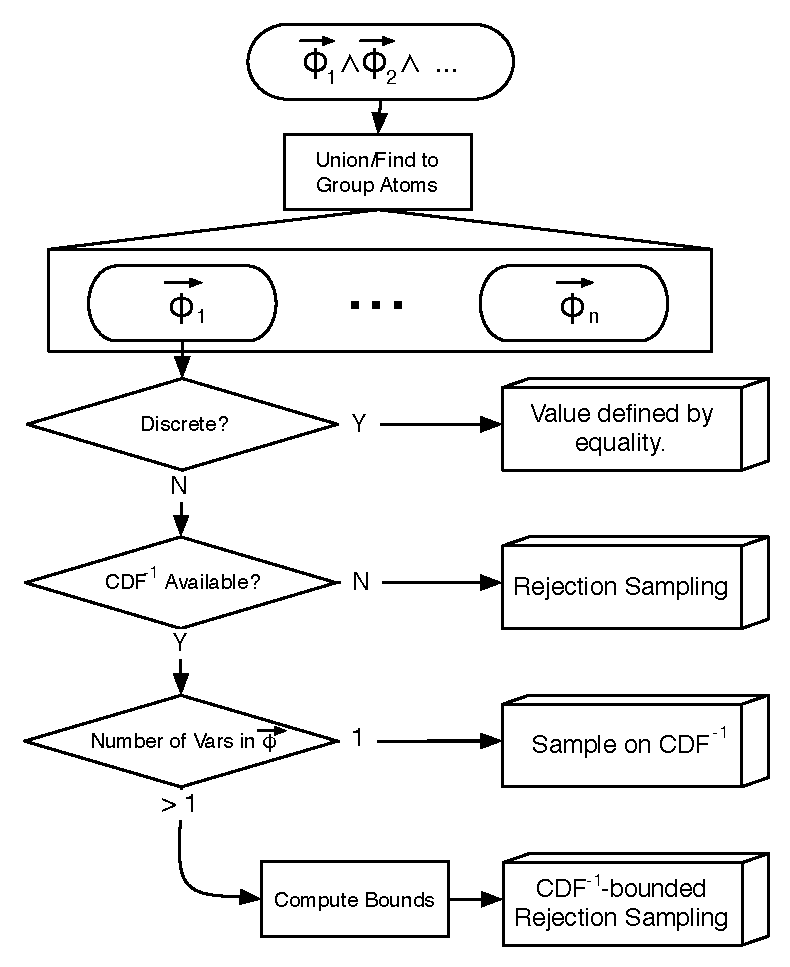
\includegraphics{graphics/sampling_decision.pdf}}
\caption{The constrained sampling decision process}
\label{fig:sample_decision}
\end{center}
\end{figure}
} % end nop

The  most  straightforward approach  to  this  problem  is to  perform
rejection sampling; sample sets  are repeatedly generated until one is
found  that  satisfies  the   constraint  formula.   However,  as  the
probability  of satisfying  all  of  the atoms  drops,  the number  of
rejected  samples  grows.  Thus  the  cost  of  rejection sampling  is
inversely proportional to the probability of satisfying all the atoms.

If the inverse  CDF is available for a given variable,  it may be used
to rapidly generate samples  within specified bounds.  The inverse CDF
is effectively a mapping from  the domain $(0,1)$ to the corresponding
value  in  the given  distribution.   Furthermore,  the CDF  increases
monotonically.
$$[x > y] \rightarrow \left[CDF^{-1}(x) > CDF^{-1}(y)\right]$$

Thus, to obtain samples constrained  to  $(lower, upper)$, we
sample  $CDF^{-1}(X)$  where X  is  chosen  uniformly  from the  range
$(CDF(lower), CDF(upper))$.   In the  unlikely event that  the inverse
CDF is  available, but  the CDF  is not, this  technique may  still be
used.  Instead of sampling  from the range $(CDF(lower), CDF(upper))$,
we instead sample  $x \in (L,H)$ where $L$ is  initialized to $0$, and
$H$ is initialized to $1$.  If $CDF^{-1}(x) \leq lower$ we set $L = x$
and try again.  Similarly, if $CDF^{-1}(x)  \geq upper$ we set $H = x$
and  try again.   In  this way,  we  effectively learn  the values  of
$CDF(lower)$ and $CDF(upper)$.

When the inverse CDF is not available, naive sampling is typically the
most  efficient  approach.  The  probability  of  a  set of  variables
satisfying  a set  of atoms  is increased  as the  number of  atoms is
reduced.  As in conjunctive integration, it is possible to improve the
success  rate  by  separately  generating  samples  for  each  minimal
independent  subset.  Because  the  subsets are  smaller,  it is  less
likely that a sample will  need to be discarded.  Furthermore, because
fewer variables are being  sampled for each subset, less computational
effort is wasted generating invalid samples.

\subsection{MCMC Sampling}
\label{subsec:MCMC}
A final alternative available to PIP, is the
Metropolis  algorithm \cite{metropolis}.   Starting from  an arbitrary
point within the sample space,  this algorithm performs a random walk.
Steps  are  sampled  from  a  multivariate  normal  distribution,  and
rejection sampling  is used  to weight the  walk towards  regions with
higher  probability  densities.  Samples  taken  at regular  intervals
during the random walk may be used as samples of the distribution.

Because the Metropolis  algorithm uses relative probability densities,
it is possible to use a density function that has not been normalized.
Thus, regions of  space that do not satisfy the  clause are assigned 0
density; the random walk never enters these regions.

The Metropolis algorithm has an  expensive startup cost, as there is a
lengthy  `burn-in' period  while  it generates  a sufficiently  random
initial  value.  Despite  this startup  cost, the  algorithm typically
requires only a relatively small  number of steps between each sample.
Consequently,   the  Metropolis  algorithm   is  ideally   suited  for
generating large numbers of samples  when the CDF is not available and
the probability of sampling a given value is small.

It necessary to parametrize the normal distribution used to select the
next step in the random walk.  Specifically, the standard deviation is
highly dependent on the distribution being sampled from;  If the value selected is
too small,  steps taken  by the  algorithm will be  too small  and the
number  of  steps required  to  generate  independent samples  becomes
large.   If  the value  selected  is  too  large, the  algorithm  will
frequently attempt to leave the  constraint bounds and thus many steps
will be rejected.

PIP uses the burn-in phase to select an appropriate standard deviation
for  each  dimension.   Prior  to  sampling, PIP  performs  a  dynamic
standard deviation  computation.  Steps are limited  to movement along
one axis;  thus only one  variable contributes to the  step direction.
If  the step  is rejected,  the standard  deviation for  that  axis is
lowered by a  constant factor.  If the step  is accepted, the standard
deviation is raised by a  constant factor.  These factors are selected
such  that the  standard  deviation  converges to  a  point where  the
acceptance-rejection ratio falls in  the commonly accepted ideal range
of  $0.1-0.4$\cite{numericalrecipes}.  The  dynamic standard  deviation computation  does not
replace the burn-in  phase, but instead reduces the  number of burn-in
steps required.



\subsection{Computing Confidences}
\label{subsec:cint}


Computing the confidence of a row in the C-Table; ie, computing the 
probability that the conjunction $\phi$ of the row's condition atoms, 
is equivalent to computing
\[
\sum_{\vec{x}} \int_{\vec{y}} p(\vec{x}, \vec{y}) \cdot \chi_\phi(\vec{x},\vec{y}) \; d\vec{y}.
\]
This integral may be naively estimated via Monte Carlo sampling as
described in Section \ref{sec:montecarlo}.
The difficulty is twofold: First, it must be possible to sample from $p$.
Second, enforcing $\chi_\phi$ requires rejection sampling, which can be
very inefficient if $\phi$ is selective.




%ck: where is the optimization? which choice do we have?
\nop{
All relevant conditions are  known prior to integration.  This advance
knowledge  may be  used to  produce more  accurate estimates  at lower
costs.

The first  optimization stems  from the observation  that the  cost of
Monte Carlo integration is inversely  proportional to the scale of the
value being  computed; in order  to achieve estimates  with equivalent
precision\footnote{It   is  important   to  distinguish   between  two
different precision metrics: the  number of significant figures in the
result as  opposed to the number  of decimal places.   This paper uses
the former  metric, referring to  the latter as  the \textit{absolute}
precision.} fewer iterations are required if the value being estimated
is large.   When estimating the  expectation $E[g]$, the scale  of the
computed  probability drops  as  the number  of constrained  variables
grows.  Thus, fewer  total samples will be needed  to achieve a target
precision  if  it is  possible  to  sample  subsets of  the  variables
independently.
} % end nop


{\bf Exploiting independence.}
To minimize the number of variables being integrated at one time, PIP first subdivides constraint atoms into minimal independent subsets.  Two constraint subsets are independent if their member atoms have no variables in common.  When determining subset independence, composite random variables (for instance, defined by artithmetic expressions over random variables) are treated as the set of all of their component variables.  By definition, atoms in each subset are independent.  Thus, the probability of each subset may be computed independently as well; the overall probability is the product of the independent probabilities.  For example, consider the one row c-table 
\[
\begin{tabular}{c|c}
R & $\phi_2$ \\
\hline
& $(X > 4) \wedge ([X\cdot Z] > Y) \wedge (A < 6)$ \\
\end{tabular}
\]
In this case, the atoms $(X > 4)$ and $([X\cdot Z] > Y)$ form one minimal independent subset, while $(A < 6)$ forms another.

Because condition atoms describing discrete variables are all of the form $Var = Val$, discrete variables are handled trivially.  Inconsistent values have already been removed, so the probability for the entire subgroup is the probability of the listed variable assignment.

The simplest subset of continuous atoms is one that references only one variable.  In this case, the atoms in the set provide constant upper or lower bounds, and the integration problem may be solved by evaluating the variable's CDF at the tightest upper and lower bounds.  If the CDF is not available or if it is not possible to derive tight bounds on the CDF, PIP can still integrate via Monte Carlo sampling.  In the one-variable case, numerical integration of the variable's PDF could also be used where an extremely precise answer is required.

{\bf Sampling using inverse CDFs}.
With more than two variables in the independent subset, Monte Carlo sampling becomes the most effective way of estimating the subset's probability.  As has already been noted, Monte Carlo techniques perform poorly if the value being computed is small.  However, in some cases PIP may be able to use a variable's CDF to reduce the sampling area.  

As discussed in Section \ref{subsec:csampling}, inverted CDFs allow efficient sampling of bounded variables.  For each variable in the subset where both a CDF and an inverted CDF are available, PIP computes the variable's upper and lower bounds from the atoms in the subset.  This includes both direct constraints of the form $X > C$, where $X$ is bounded on the bottom by $C$, and pairwise constraints of the form $X + Y < C_1$ and $X - Y < C_2$, where $X$ is bounded on the top by $\frac{C_1+C_2}{2}$.  

Applied to all the variables in the subset that have both a CDF and an inverted CDF, this process creates a hyper-rectangular bounding box in the sample space.  Because rectangular bounds are independent, the probability of a sample falling within the bounds can be computed independently for each variable as above.  Finally, Monte Carlo integration is performed, but only within the subspace.
%
%ck: i think not
%The result of this integration is normalized by the probability of a sample
%falling within the rectangular bounds.
%
Because  sampling is  constrained  to the  bounded  area, Monte  Carlo
integration avoid rejection sampling, and requires fewer samples for a
higher precision.

This  process is  only possible  if rectangular  bounds on  the sample
space exist.  However, it is  most useful when the probability density
contained within the atoms is  small.  Though it is possible to define
non-convex   constraint   atoms,   all   linear  atoms   are   convex.
Furthermore, the space  defined by the conjunction of  a set of convex
atoms is itself  convex.  Thus, anecdotally it is possible to
define a bounding box containing no less than half of the area defined
by the constraints.


There are  cases where bounds are insufficient.   For example, concave
atoms  are   not  likely   to  admit  effective   rectangular  bounds.
Similarly, even though a bounding box  covers no less than half of the
volume of a contiguous convex constraint area, the  bulk of the  probability mass may
still lie  outside of the constrained  sample area.  In  such cases, a
recursive technique may be applied.

The  bounding box  is first  subdivided into  smaller  regions.  Monte
Carlo integration  is performed on the  region twice, but  with only a
small number of iterations apiece.  If the two results agree to within
the  desired  precision, integration  stops  and  the  average of  the
results is multiplied by the  probability of a sample falling into the
sampling region.  If the  two results differ significantly, the region
is further subdivided and the algorithm recurses on each sub-region.

Because the  recursive cutoff is determined by  the estimated accuracy
of the  result, this  algorithm will not  recurse on regions  that are
entirely   within  or   outside  of   the  constrained   sample  area.
Consequently, the majority of  samples generated by the algorithm will
be  put towards estimating  relatively high  values where  Monte Carlo
integration is most effective.


